
%% bare_conf.tex
%% V1.3
%% 2007/01/11
%% by Michael Shell
%% See:
%% http://www.michaelshell.org/
%% for current contact information.
%%
%% This is a skeleton file demonstrating the use of IEEEtran.cls
%% (requires IEEEtran.cls version 1.7 or later) with an IEEE conference paper.
%%
%% Support sites:
%% http://www.michaelshell.org/tex/ieeetran/
%% http://www.ctan.org/tex-archive/macros/latex/contrib/IEEEtran/
%% and
%% http://www.ieee.org/

%%*************************************************************************
%% Legal Notice:
%% This code is offered as-is without any warranty either expressed or
%% implied; without even the implied warranty of MERCHANTABILITY or
%% FITNESS FOR A PARTICULAR PURPOSE! 
%% User assumes all risk.
%% In no event shall IEEE or any contributor to this code be liable for
%% any damages or losses, including, but not limited to, incidental,
%% consequential, or any other damages, resulting from the use or misuse
%% of any information contained here.
%%
%% All comments are the opinions of their respective authors and are not
%% necessarily endorsed by the IEEE.
%%
%% This work is distributed under the LaTeX Project Public License (LPPL)
%% ( http://www.latex-project.org/ ) version 1.3, and may be freely used,
%% distributed and modified. A copy of the LPPL, version 1.3, is included
%% in the base LaTeX documentation of all distributions of LaTeX released
%% 2003/12/01 or later.
%% Retain all contribution notices and credits.
%% ** Modified files should be clearly indicated as such, including  **
%% ** renaming them and changing author support contact information. **
%%
%% File list of work: IEEEtran.cls, IEEEtran_HOWTO.pdf, bare_adv.tex,
%%                    bare_conf.tex, bare_jrnl.tex, bare_jrnl_compsoc.tex
%%*************************************************************************

% *** Authors should verify (and, if needed, correct) their LaTeX system  ***
% *** with the testflow diagnostic prior to trusting their LaTeX platform ***
% *** with production work. IEEE's font choices can trigger bugs that do  ***
% *** not appear when using other class files.                            ***
% The testflow support page is at:
% http://www.michaelshell.org/tex/testflow/



% Note that the a4paper option is mainly intended so that authors in
% countries using A4 can easily print to A4 and see how their papers will
% look in print - the typesetting of the document will not typically be
% affected with changes in paper size (but the bottom and side margins will).
% Use the testflow package mentioned above to verify correct handling of
% both paper sizes by the user's LaTeX system.
%
% Also note that the "draftcls" or "draftclsnofoot", not "draft", option
% should be used if it is desired that the figures are to be displayed in
% draft mode.
%
\documentclass[conference]{IEEEtran}
\usepackage{blindtext, graphicx}
% Add the compsoc option for Computer Society conferences.
%
% If IEEEtran.cls has not been installed into the LaTeX system files,
% manually specify the path to it like:
% \documentclass[conference]{../sty/IEEEtran}
% Some very useful LaTeX packages include:
% (uncomment the ones you want to load)


% *** MISC UTILITY PACKAGES ***
%
%\usepackage{ifpdf}
% Heiko Oberdiek's ifpdf.sty is very useful if you need conditional
% compilation based on whether the output is pdf or dvi.
% usage:
% \ifpdf
%   % pdf code
% \else
%   % dvi code
% \fi
% The latest version of ifpdf.sty can be obtained from:
% http://www.ctan.org/tex-archive/macros/latex/contrib/oberdiek/
% Also, note that IEEEtran.cls V1.7 and later provides a builtin
% \ifCLASSINFOpdf conditional that works the same way.
% When switching from latex to pdflatex and vice-versa, the compiler may
% have to be run twice to clear warning/error messages.






% *** CITATION PACKAGES ***
%
%\usepackage{cite}
% cite.sty was written by Donald Arseneau
% V1.6 and later of IEEEtran pre-defines the format of the cite.sty package
% \cite{} output to follow that of IEEE. Loading the cite package will
% result in citation numbers being automatically sorted and properly
% "compressed/ranged". e.g., [1], [9], [2], [7], [5], [6] without using
% cite.sty will become [1], [2], [5]--[7], [9] using cite.sty. cite.sty's
% \cite will automatically add leading space, if needed. Use cite.sty's
% noadjust option (cite.sty V3.8 and later) if you want to turn this off.
% cite.sty is already installed on most LaTeX systems. Be sure and use
% version 4.0 (2003-05-27) and later if using hyperref.sty. cite.sty does
% not currently provide for hyperlinked citations.
% The latest version can be obtained at:
% http://www.ctan.org/tex-archive/macros/latex/contrib/cite/
% The documentation is contained in the cite.sty file itself.






% *** GRAPHICS RELATED PACKAGES ***
%
\ifCLASSINFOpdf
  % \usepackage[pdftex]{graphicx}
  % declare the path(s) where your graphic files are
  % \graphicspath{{../pdf/}{../jpeg/}}
  % and their extensions so you won't have to specify these with
  % every instance of \includegraphics
  % \DeclareGraphicsExtensions{.pdf,.jpeg,.png}
\else
  % or other class option (dvipsone, dvipdf, if not using dvips). graphicx
  % will default to the driver specified in the system graphics.cfg if no
  % driver is specified.
  % \usepackage[dvips]{graphicx}
  % declare the path(s) where your graphic files are
  % \graphicspath{{../eps/}}
  % and their extensions so you won't have to specify these with
  % every instance of \includegraphics
  % \DeclareGraphicsExtensions{.eps}
\fi
% graphicx was written by David Carlisle and Sebastian Rahtz. It is
% required if you want graphics, photos, etc. graphicx.sty is already
% installed on most LaTeX systems. The latest version and documentation can
% be obtained at: 
% http://www.ctan.org/tex-archive/macros/latex/required/graphics/
% Another good source of documentation is "Using Imported Graphics in
% LaTeX2e" by Keith Reckdahl which can be found as epslatex.ps or
% epslatex.pdf at: http://www.ctan.org/tex-archive/info/
%
% latex, and pdflatex in dvi mode, support graphics in encapsulated
% postscript (.eps) format. pdflatex in pdf mode supports graphics
% in .pdf, .jpeg, .png and .mps (metapost) formats. Users should ensure
% that all non-photo figures use a vector format (.eps, .pdf, .mps) and
% not a bitmapped formats (.jpeg, .png). IEEE frowns on bitmapped formats
% which can result in "jaggedy"/blurry rendering of lines and letters as
% well as large increases in file sizes.
%
% You can find documentation about the pdfTeX application at:
% http://www.tug.org/applications/pdftex





% *** MATH PACKAGES ***
%
%\usepackage[cmex10]{amsmath}
% A popular package from the American Mathematical Society that provides
% many useful and powerful commands for dealing with mathematics. If using
% it, be sure to load this package with the cmex10 option to ensure that
% only type 1 fonts will utilized at all point sizes. Without this option,
% it is possible that some math symbols, particularly those within
% footnotes, will be rendered in bitmap form which will result in a
% document that can not be IEEE Xplore compliant!
%
% Also, note that the amsmath package sets \interdisplaylinepenalty to 10000
% thus preventing page breaks from occurring within multiline equations. Use:
%\interdisplaylinepenalty=2500
% after loading amsmath to restore such page breaks as IEEEtran.cls normally
% does. amsmath.sty is already installed on most LaTeX systems. The latest
% version and documentation can be obtained at:
% http://www.ctan.org/tex-archive/macros/latex/required/amslatex/math/





% *** SPECIALIZED LIST PACKAGES ***
%
%\usepackage{algorithmic}
% algorithmic.sty was written by Peter Williams and Rogerio Brito.
% This package provides an algorithmic environment fo describing algorithms.
% You can use the algorithmic environment in-text or within a figure
% environment to provide for a floating algorithm. Do NOT use the algorithm
% floating environment provided by algorithm.sty (by the same authors) or
% algorithm2e.sty (by Christophe Fiorio) as IEEE does not use dedicated
% algorithm float types and packages that provide these will not provide
% correct IEEE style captions. The latest version and documentation of
% algorithmic.sty can be obtained at:
% http://www.ctan.org/tex-archive/macros/latex/contrib/algorithms/
% There is also a support site at:
% http://algorithms.berlios.de/index.html
% Also of interest may be the (relatively newer and more customizable)
% algorithmicx.sty package by Szasz Janos:
% http://www.ctan.org/tex-archive/macros/latex/contrib/algorithmicx/




% *** ALIGNMENT PACKAGES ***
%
%\usepackage{array}
% Frank Mittelbach's and David Carlisle's array.sty patches and improves
% the standard LaTeX2e array and tabular environments to provide better
% appearance and additional user controls. As the default LaTeX2e table
% generation code is lacking to the point of almost being broken with
% respect to the quality of the end results, all users are strongly
% advised to use an enhanced (at the very least that provided by array.sty)
% set of table tools. array.sty is already installed on most systems. The
% latest version and documentation can be obtained at:
% http://www.ctan.org/tex-archive/macros/latex/required/tools/


%\usepackage{mdwmath}
%\usepackage{mdwtab}
% Also highly recommended is Mark Wooding's extremely powerful MDW tools,
% especially mdwmath.sty and mdwtab.sty which are used to format equations
% and tables, respectively. The MDWtools set is already installed on most
% LaTeX systems. The lastest version and documentation is available at:
% http://www.ctan.org/tex-archive/macros/latex/contrib/mdwtools/


% IEEEtran contains the IEEEeqnarray family of commands that can be used to
% generate multiline equations as well as matrices, tables, etc., of high
% quality.


%\usepackage{eqparbox}
% Also of notable interest is Scott Pakin's eqparbox package for creating
% (automatically sized) equal width boxes - aka "natural width parboxes".
% Available at:
% http://www.ctan.org/tex-archive/macros/latex/contrib/eqparbox/





% *** SUBFIGURE PACKAGES ***
%\usepackage[tight,footnotesize]{subfigure}
% subfigure.sty was written by Steven Douglas Cochran. This package makes it
% easy to put subfigures in your figures. e.g., "Figure 1a and 1b". For IEEE
% work, it is a good idea to load it with the tight package option to reduce
% the amount of white space around the subfigures. subfigure.sty is already
% installed on most LaTeX systems. The latest version and documentation can
% be obtained at:
% http://www.ctan.org/tex-archive/obsolete/macros/latex/contrib/subfigure/
% subfigure.sty has been superceeded by subfig.sty.



%\usepackage[caption=false]{caption}
%\usepackage[font=footnotesize]{subfig}
% subfig.sty, also written by Steven Douglas Cochran, is the modern
% replacement for subfigure.sty. However, subfig.sty requires and
% automatically loads Axel Sommerfeldt's caption.sty which will override
% IEEEtran.cls handling of captions and this will result in nonIEEE style
% figure/table captions. To prevent this problem, be sure and preload
% caption.sty with its "caption=false" package option. This is will preserve
% IEEEtran.cls handing of captions. Version 1.3 (2005/06/28) and later 
% (recommended due to many improvements over 1.2) of subfig.sty supports
% the caption=false option directly:
%\usepackage[caption=false,font=footnotesize]{subfig}
%
% The latest version and documentation can be obtained at:
% http://www.ctan.org/tex-archive/macros/latex/contrib/subfig/
% The latest version and documentation of caption.sty can be obtained at:
% http://www.ctan.org/tex-archive/macros/latex/contrib/caption/




% *** FLOAT PACKAGES ***
%
%\usepackage{fixltx2e}
% fixltx2e, the successor to the earlier fix2col.sty, was written by
% Frank Mittelbach and David Carlisle. This package corrects a few problems
% in the LaTeX2e kernel, the most notable of which is that in current
% LaTeX2e releases, the ordering of single and double column floats is not
% guaranteed to be preserved. Thus, an unpatched LaTeX2e can allow a
% single column figure to be placed prior to an earlier double column
% figure. The latest version and documentation can be found at:
% http://www.ctan.org/tex-archive/macros/latex/base/



%\usepackage{stfloats}
% stfloats.sty was written by Sigitas Tolusis. This package gives LaTeX2e
% the ability to do double column floats at the bottom of the page as well
% as the top. (e.g., "\begin{figure*}[!b]" is not normally possible in
% LaTeX2e). It also provides a command:
%\fnbelowfloat
% to enable the placement of footnotes below bottom floats (the standard
% LaTeX2e kernel puts them above bottom floats). This is an invasive package
% which rewrites many portions of the LaTeX2e float routines. It may not work
% with other packages that modify the LaTeX2e float routines. The latest
% version and documentation can be obtained at:
% http://www.ctan.org/tex-archive/macros/latex/contrib/sttools/
% Documentation is contained in the stfloats.sty comments as well as in the
% presfull.pdf file. Do not use the stfloats baselinefloat ability as IEEE
% does not allow \baselineskip to stretch. Authors submitting work to the
% IEEE should note that IEEE rarely uses double column equations and
% that authors should try to avoid such use. Do not be tempted to use the
% cuted.sty or midfloat.sty packages (also by Sigitas Tolusis) as IEEE does
% not format its papers in such ways.


% *** PDF, URL AND HYPERLINK PACKAGES ***
%
%\usepackage{url}
% url.sty was written by Donald Arseneau. It provides better support for
% handling and breaking URLs. url.sty is already installed on most LaTeX
% systems. The latest version can be obtained at:
% http://www.ctan.org/tex-archive/macros/latex/contrib/misc/
% Read the url.sty source comments for usage information. Basically,
% \url{my_url_here}.





% *** Do not adjust lengths that control margins, column widths, etc. ***
% *** Do not use packages that alter fonts (such as pslatex).         ***
% There should be no need to do such things with IEEEtran.cls V1.6 and later.
% (Unless specifically asked to do so by the journal or conference you plan
% to submit to, of course. )


% correct bad hyphenation here
\usepackage[english]{babel} % English language/hyphenation
\usepackage{array}
\usepackage{multirow}
\usepackage{amsmath}
\numberwithin{equation}{section}
\numberwithin{figure}{section}
\numberwithin{table}{section}
\usepackage{caption}

\begin{document}


%
% paper title
% can use linebreaks \\ within to get better formatting as desired
\title{Emotion Analysis using Word Embedding and Neural Network}

\author{\IEEEauthorblockN{Arora, Pragya\IEEEauthorrefmark{1},
Ghai, Piyush\IEEEauthorrefmark{2}, Gupta, Harsh\IEEEauthorrefmark{3} and
Ramkrishnan, Navnith\IEEEauthorrefmark{4}}
\IEEEauthorblockA{Department of Computer Science \& Engineering,
The Ohio State University\\
Columbus, OH 43202\\
Email: \IEEEauthorrefmark{1}arora.170@osu.edu,
\IEEEauthorrefmark{2}ghai.8@osu.edu,
\IEEEauthorrefmark{3}gupta.749@osu.edu,
\IEEEauthorrefmark{4}ramkrishnan.1@osu.edu}}
\maketitle


\begin{abstract}
%\boldmath
Human computer interaction and its applications such as chat bots and voice assistants  will be more natural if computers are able to perceive and respond to human non-verbal communication such as emotions. Although a lot of work has been done in the field of sentiment analysis but relatively little work has been done to detect emotions such as joy, anger, surprise in a text. This paper tries to extract the embedding based on words from a text document and apply state of the art neural network techniques to predict what emotion the writer wants to convey from the text. We experimented on two approaches along with a baseline approach to extract emotion decision using word embeddings. We used ISEAR dataset to label seven emotions. The emotion classes are sadness, anger, joy, shame, disgust, guilt and fear. The results reveals that the system based on Long Short Term Memory (LSTM) gave better performance than the system based on Convolution Neural Networks (CNN) for the emotions considered. Results also show when our feature engineered vectors and Word2Vec were jointly learned, the performance and the robustness of the emotion recognition system improve measurably. 
\end{abstract}
% IEEEtran.cls defaults to using nonbold math in the Abstract.
% This preserves the distinction between vectors and scalars. However,
% if the journal you are submitting to favors bold math in the abstract,
% then you can use LaTeX's standard command \boldmath at the very start
% of the abstract to achieve this. Many IEEE journals frown on math
% in the abstract anyway.

% Note that keywords are not normally used for peerreview papers.
\section{Introduction}
Emotion Analysis and Identification is the cornerstone of recent study in the fields of neuroscience, psychology, cognitive sciences and behavioral science as they serve as a good indicator of human nature. The major techniques to predict emotion are on the basis of supervised learning through hand annotated data to train and build predictive models. Despite these models achieving good results, the availability of large sets of tagged data and transferability of performance on different domains have been deterrents. 

In this paper, we use the ISEAR (International Survey on Emotion Antecedents and Reactions) Dataset \cite{iseardataset}, which comprises of 7516 sentences and seven emotion categories including : \textit{Anger}, \textit{Disgust}, \textit{Fear}, \textit{Guilt}, \textit{Joy}, \textit{Sadness}, \textit{Shame}. 

\section{Related Work}\label{sec:page-layout}
This section expands on lexical resources and research work supporting work on Emotion Analysis from a corpora and gives a brief about other such novel methodologies. 


\subsection{Lexical Resources}\label{sec:formatting}
Lexical resources have long been used for emotion and opinion analysis. Strides in lexical resources began with a list of 1,336 hand annottated adjectives. Other advances include WordNet - Affect which comprises of hierarchial domain of affective labels. In the sphere of sentiment, SentiWordNet \cite{sentiword} accounts for opinion related properties of text. SentiFul database further assisted with automatic generated lexicons. Researchers came up with subjectivity lexicon which accounted for 8,000 words. 


%% Notice that paragraph breaks are done with a blank line between paragraphs


\subsection{Emotion Detection Approaches
}\label{sec:formatting-text}

Classification of Emotion can be done based on the presence or absence of affective lexicons. Further distinction can be done based on keywords, linguistic rules and the application of machine learning approaches. 
\subsubsection{ Keyword-based Techniques using Affective Lexicons}\label{sec:cap-num}
Keyword-based approach is the most primitive form implemented at the base word level and such models are incapable of handling affect expressed by interrelated words. 

\subsubsection{Linguistic Rules-based Approaches}\label{sec:positioning}
Computational linguists define linguistic structure based on a set of rules. 

\begin{itemize}
\item Rule-based approaches with Affect Lexicons: Classification of emotions in news headlines is the main purpose behind the ESNA System \cite{esna}. UPAR7 has hand annotated seed words in emotion lists aided by rules which outline the main context and use dependency graphs to boost emotion ratings. Recent strides in rule-based approaches recognize up to nine emotions. General Inquirer and Wordnet explore the effect of conjuncts using techniques of syntax and lexical resources. The definition and deciphering of complex structures are well handled in comparison to designing and modification by these approaches. One flaw in affect lexicons is the inflexibility to handle emotions not listed. 

\item Rule-based approaches without Affect Lexicons: In the absence of affect lexicons, semantic structure of language is the crux. Metaphorical data further aid in emotion recognition from text. These methods are flexible and relevant in real world implementation. The rules are structured and represent the extracted data in concurrence with the source. 

\end{itemize}


\subsection{Machine Learning Approaches}\label{sec:formatting-text}
Machine learning techniques which can be broadly classified as supervised and unsupervised machine learning has been deployed to overcome the short falls of rule based methods which do not take into account all the possibly corner cases and is short at capturing the evolution of writing texts by human.

\subsubsection{Supervised machine learning with affect lexicons}\label{sec:cap-num}
Under this approach a database is created for the affect words where each affect word is divided into smaller classes to make it a find grained resource and now this resource is used for multi class classification of emotions. Models like Support Vector Machine is used under this technique. For supervised learning the problem is that we need a lot of data to train the classifier and then the trained model works on a domain specific data set, which is its disadvantage.

\subsubsection{Supervised machine learning without affect lexicons}\label{sec:positioning}
Using a BOW approach or a tf-idf approach works well even if we don't consider the affect words while training the model. Even this kind of technique suffers from the bias of giving good results only for data coming from a specific origin.

\subsubsection{Unsupervised machine learning with affect lexicons}\label{sec:positioning}
An evaluation of two unsupervised techniques using WordNet-Affect exploited a vector space model and a number of dimensionality reduction methods. News headlines have been classified using simple heuristics and more refined algorithms (e.g., similarity in a latent semantic space).

\subsubsection{Unsupervised machine learning without affect lexicons}\label{sec:positioning} Latent Semantic analysis single word approach which compares the similarity between text documents and all the emotion labels along with LSA synsets and WordNet synsets.



\section{Proposed Approach}\label{sec:fig-tables}
In our approach we have modeled our framework to run on state of the art machine learning algorithms and learn the context of the data using their vectors from Word2Vec \cite{word2vec} \& GloveVec \cite{glove}. After the model is trained on several hyper parameters we tested our model on unseen data set and calculated the accuracy which is better than baseline given in related papers. Our emotion recognition algorithm includes three main components: preprocessing, semantic transformation of Word embedding and application of Machine Learning algorithm. 

\subsection{Preprocessing \& Word Embedding}\label{sec:cap-num}
We used ISEAR data set to test our model. This dataset has sentences tagged with an emotion label. The preprocessing task consists of word level parsing along with tokenization and stemming which cleans the text document of unwanted stop words which don't relate to emotion. This enables us to extract the relevant affect-bearing words and the syntactic dependencies between words. The next step is to perform word-level analysis by computing a word embedding for the affect-bearing words by using the glove vector and also alternately learning the word embedding for this model by itself. \\

The transcript of the text documents were extracted, converted to all lower case characters. We did not remove punctuations here, because our intuition was that these punctuation marks can have a bearing on the emotion classification of a sentence. We then preprocessed the sentences using NLTK Tokenizer to give a list of tokens. This list of tokens was converted into a word embedding using Word2Vec model for (CNN) and Glove model (LSTM). For each word a 300 dimensional embedding was created. This could have been tweaked, however for simplicity, we stuck with a 300 dimensional vector. \cite{lstm2}


\subsection{Application of Machine Learning Techniques}\label{sec:colour-illustrations}
After the word embeddings are prepared, the word vectors are given as an input to our neural network models. The model is then trained on several hyper parameters like the number of epochs, number of layers, drop out probability, activation function, loss function, optimizer and learning rate.

\subsubsection {Long Short Term Memory(LSTM)\cite{lstm}}
We have mapped each sentence into a real vector domain called GloVe embedding. This is a technique where words are encoded as real-valued vectors in a high dimensional space, where the similarity between words in terms of meaning translates to closeness in the vector space.
We have mapped each word into 300 length vector and there are around 9000 unique words so a matrix of 9000x300 is created. This positive integer representation of words is fed into Embedding layer which converts it into word embedding.
The first layer is the Embedded layer that uses 300 length vectors to represent each word. The next layer is the LSTM layer with 128 memory units and 0.6 dropout to input and recurrent connections of the memory units with LSTM. Finally, because this is a classification problem we use a Dense output layer with seven neurons, a softmax activation function with categorical crossentropy and ADAM optimizer. A large batch size of 128 reviews is used to space out weight updates.  We observed that applying dropout as a parameter to the LSTM Model led to an increase in the accuracy.
\begin{figure}
  \centering
  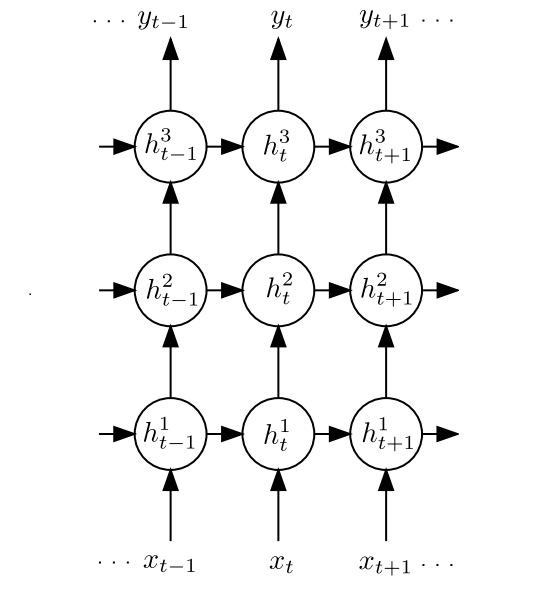
\includegraphics[width=\columnwidth]{LSTM_image}
  \caption{LSTM model for word embedding}
    \label{lstm}
\end{figure}

In Figure \ref{lstm} xt's are word embedding which is 300 dimensional vector and y's are the output from the output layer. In our LSTM model we have three hidden layers which included embedding layer, lstm layer, dense output layer. The output is passed through a softmax function which gives us a 7 dimensional vector as the output. 


\subsubsection{Convolutional Neural Networks}
For implementing CNN, we implemented a model similar to Kim Yoon's Convolutional Neural Networks for Sentence Classification \cite{kimyoon} \cite{wildmlcnn}.
The CNN architecture used by us for the emotion analysis task is given in Figure \ref{fig_cnn}. The network used by us works roughly as follows : 
\begin{itemize}
\item The first layer embeds the words into lower dimensional vectors.
\item The next layer performs convolutions over the embeddings from the first layer using multiple filter sizes.
\item Next up, we max-pool the result of the convolutional layer into a feature vector, over which we add dropout regularization and use softmax at the output layer to classify the result.
\end{itemize}


\begin{figure}
  \centering
  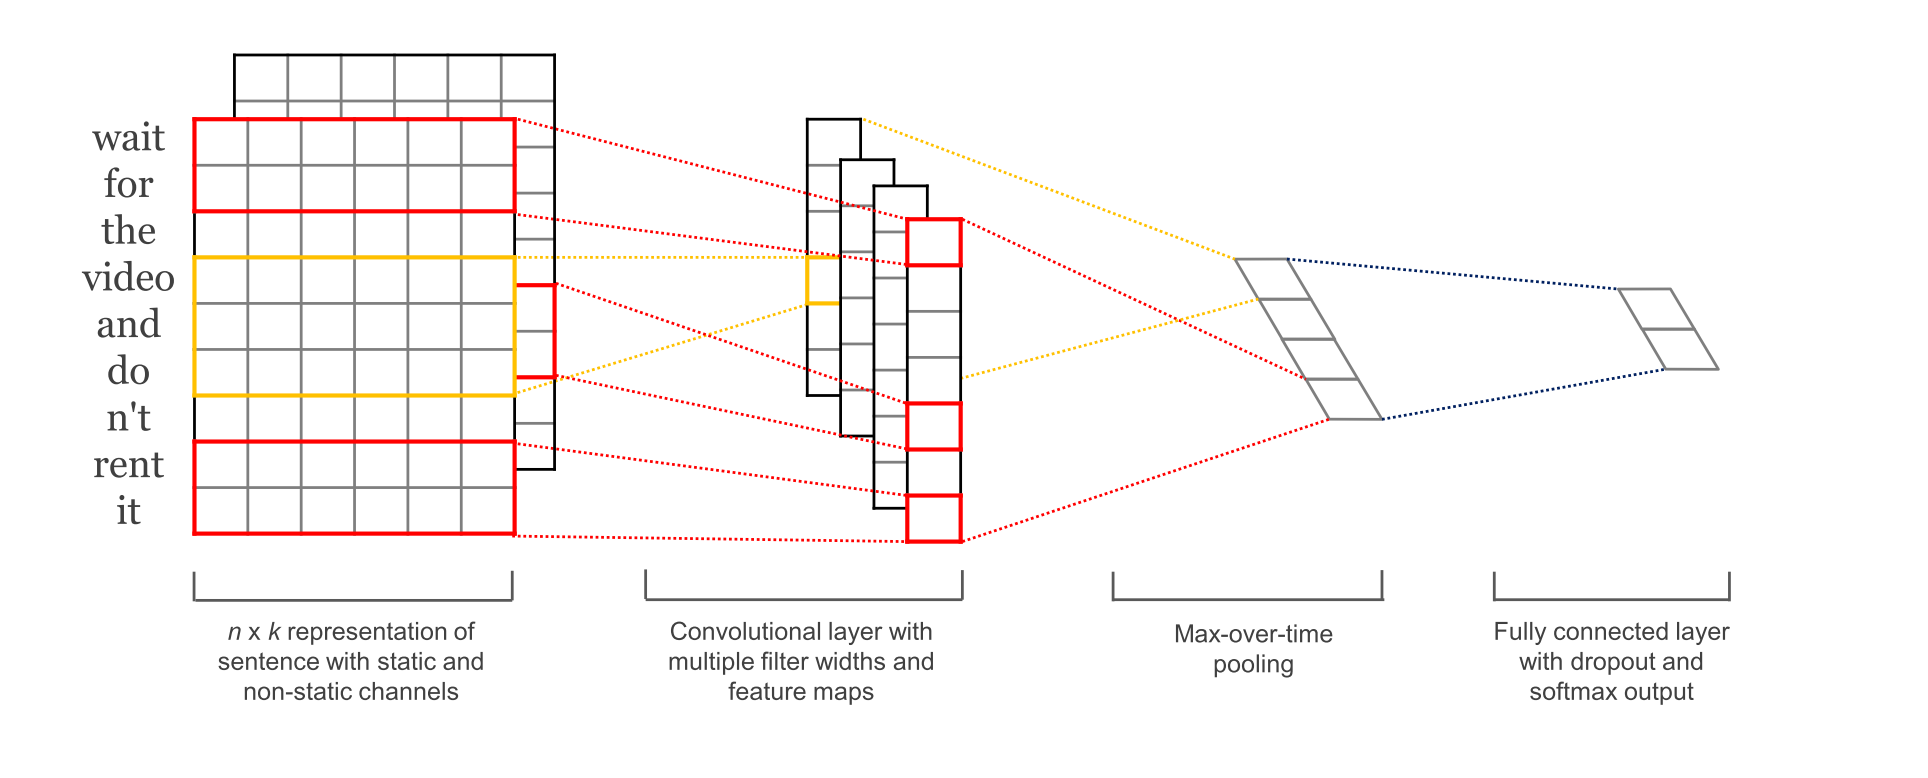
\includegraphics[width=\columnwidth]{cnn_arch}
  \caption{CNN model}
    \label{fig_cnn}
\end{figure}

\section{Experimental Setup}
We run our dataset on several models. 
All our models presented below were evaluated on a 70-30 train-test split and 90-10 train-dev set split.
\subsection{Dumb Baseline}
The dumb baseline model, predicts the emotions at random for a text from the given 7 emotion labels. This approach, not too surprisingly performs poorly.

\subsection{Multinomial Na{\"i}ve Bayes}
We used TFIDF Vectorizer for Multinomial Na{\"i}ve Bayes which gives us an accuracy of 0.567 on the test dataset. We also used Multinomial Na{\"i}ve Bayes with a Bag of Words approach. This performed slightly lower than the TFIDF Vectorizer and we got an accuracy of 0.562. The results are summarized in Table \ref{tab_nb}. 

\subsection{Extra Tree Classifier}
We also used Extra tree classifier (Random Forest Classification). With this classifier we changed the word representations using Word2Vec and GloveVectors representation. After changing the word representations, TFIDF Vectorizer was used. The results were not very encouraging with this though. We achieved a maximum accuracy of 0.4313 with Glove representation of the input text. The results are summarized in Table \ref{tab_nb}.

\subsection{SVM	}
We next implemented a multi-class, one versus all classifier. The input to the SVM was a TFIDF vectorized representation of the words. The accuracy for One v/s All SVM was 0.56489. 

\begin{table}[!htb]
 \centering
 \caption{Accuracy on ISEAR Test Dataset for several algorithms}
 \label{tab_nb}
\begin{tabular}{ c c c c  } 
    \noalign{\smallskip}\hline\noalign{\smallskip}
   Model &  Processing Approach & Accuracy \\
       \noalign{\smallskip}\hline\noalign{\smallskip}
\multirow{1}{8em} {Dumb Baseline} &   -- & 0.194\\
    \noalign{\smallskip}\hline\noalign{\smallskip}
\multirow{2}{8em} {Random Forest} &   Word2Vec & 0.567021\\
&  GloveVec & 0.5625\\                
 \noalign{\smallskip}\hline\noalign{\smallskip}
\multirow{2}{8em} {Na{\"i}ve Bayes} &   With TF-IDF & 0.567021\\
&  BOW & 0.5625\\                
 \noalign{\smallskip}\hline\noalign{\smallskip}
\multirow{1}{8em} {SVM} &  One v/s All & 0.5648\\
    \noalign{\smallskip}\hline
  \end{tabular} 
\end{table}

\subsection{CNN}
For Convolutional Neural Networks, we did not use deep networks, but a shallow network and experimented with other hyperparameter tuning as well as experimenting with the word embeddings. We fixed the sequence length to 75 words. For shorter words, we padded the matrix with all zeros. 75 words as per our intuition was long enough text to judge the emotion of a sentence. The vocab size was 9000. We also varied the filter sizes, which were convolved over the words. The filter sizes were taken as \textit{3,4,5}. The number of filters were taken as 32.  In the embedding layer, we used Word2Vec representation of our dataset and we also experimented by taking random initializing of the word vectors and trained the model to learn the representations on the given inputs. For the output layer, we used softmax as the activation function. The activation used in the intermediate layers was \textit{Relu} Activation.

For hyperparameter tuning and generating accuracy, we split the training dataset into training and testing dataset present the accuracy on both dataset. The following parameters were experimented with : (The best values are indicated alongside)
\begin{itemize}
\item Number of Epochs : e  \{50\}
\item Batch Size : b    \{128\}
\item L2 Regularization : l2  \{0.60\}
\item Dropout Probability : d \{0.6\}
\end{itemize}
For word embeddings, we used pre-trained \textit{word2vec} vectors and also tried with learning embeddings from scratch. Not surprisingly, the model with word2Vec embeddings performed better in terms of overall accuracy. The results are presented in Table \ref{tab_cnn} \& Table \ref{tab_cnn2}. The training accuracies are very high suggesting overfitting for the model. The training accuracy increases, while the test accuracy decreases indicating overfitting as given in Table \ref{tab_cnn}. The same trend is followed when using with Word2Vec embeddings, however, we saw an improvement in the accuracy on the test dataset over the previous models used so far.

\begin{table}[!htb]
 \centering
 \caption{Accuracy on ISEAR Test Dataset for CNN (With No pre-trained word embeddings) with hyperparameter tuning}
 \label{tab_cnn}
\begin{tabular}{ c c c c } 
    \noalign{\smallskip}\hline\noalign{\smallskip}
	Hyperparameters & Test Accuracy & Training Accuracy \\
       \noalign{\smallskip}\hline\noalign{\smallskip}
	e=50, b=30,l2=0.3,d=0.6  & 0.5877 & 0.85230\\
	e=30, b=30,l2=0.5,d=0.6  & 0.5864 & 0.8872\\
	e=50, b=128,l2=0.6,d=0.6  & 0.5890 & 0.9053721\\
	e=40, b=128,l2=0.8,d=0.6  & 0.566489 & 0.955217\\
    \noalign{\smallskip}\hline
  \end{tabular} 
\end{table}

\begin{table}[!htb]
 \centering
 \caption{Accuracy on ISEAR Test Dataset for CNN (Using Word2Vec trained word embeddings)}
 \label{tab_cnn2}
\begin{tabular}{ c c c c } 
    \noalign{\smallskip}\hline\noalign{\smallskip}
	Hyperparameters & Test Accuracy & Training Accuracy \\
       \noalign{\smallskip}\hline\noalign{\smallskip}
	e=40, b=128,l2=0.5,d=0.6  & 0.59707 & 0.94812\\
	e=30, b=128,l2=0.3,d=0.6  & 0.60106 & 0.94634\\
	e=50, b=128,l2=0.6,d=0.6  & 0.63757 & 0.949\\
	e=50, b=128,l2=0.8,d=0.6  & 0.56909 & 0.9846\\
    \noalign{\smallskip}\hline
  \end{tabular} 
\end{table}

\subsection{LSTM}
For LSTM, we used GloveVector as word embeddings. The arhictecture for the model used has been described above. For predicting the best accuracy, the model was trained using a 90:10 training and test split, 80:20 training and test split and finally 70:30 training and test split. The validation split was fixed at 90:10 for training and dev set. The dev set was used to tune the hyperparameters. We used Adam Optimizer as the gradient descent optimization. The following were the hyperparameters of the model that we played around with : (The best values are indicated alongside.) The activation function for output layer used was Softmax activation and the loss function used was categorical cross entropy loss. Also, compared to the CNN Model, the LSTM architecture model does not seem to overfit on the given dataset, indicating that LSTM performs better.
\begin{itemize}
\item Number of Epochs : e  \{40\}
\item Activation Function ac    \{softmax\}
\item Dropout Probability : d \{0.6\}
\item Recurrent Dropout : ld \{0.6\}
\end{itemize}

\begin{table}[!htb]
 \centering
 \caption{Accuracy on ISEAR Test Dataset for LSTM (Using GloveVec trained word embeddings)}
 \label{tab_cnn}
\begin{tabular}{ c c c c } 
    \noalign{\smallskip}\hline\noalign{\smallskip}
	Hyperparameters & Test Accuracy & Training Accuracy \\
       \noalign{\smallskip}\hline\noalign{\smallskip}
	e=30,b = 128, d=0.5, ac=sigmoid  & 0.5745 & 0.8527\\
	e=50,b = 128, d=0.5, ac=sigmoid  & 0.5717 & 0.947\\
	e=30,b = 100, d=0.6, ac=softmax  & 0.5971 & 0.8952\\
	e=30,b = 256, d=0.6, ac=softmax  & 0.5984 & 0.8765\\
	e=30, LSTMDropout : 0.5, recurrent dropout:0.5    & 0.637 & 0.7437\\
	e=40, LSTMDropout : 0.6, recurrent dropout:0.6   & 0.6463 & 0.7288 \\
    \noalign{\smallskip}\hline
  \end{tabular} 
\end{table}

\section{Conclusion}
This paper addresses an important and less examined area of sentiment research on emotions, that is, emotion detection from text. The major contribution of this project is to highlight the application of neural networks to learn semantics from a data in order to identify and distinguish various types of emotions in text. We presented Long-Short Term Memory (LSTM) model which is essentially a specific kind of Recurrent Neural Networks (RNNs) and Convolutional neural network (CNN) to detect emotions from text. Experimental results show that our models perform better than other existing Machine learning approaches. Among our approaches, LSTM outperformed CNN and achieved an accuracy of 64.63\%. We tried to experiment by adding more convolutional layers to the CNN Model, but that did not boost the test accuracy a lot, instead the trend of overfitting was observed.

\section{Future Works}
Emotion detection has been studied. Although not enough time has passed to have established standards in the field, there is some consistency between the approaches, and the algorithms are continuing to increase in accuracy by using more of machine learning approach in this domain. As our future work we would like to work on better text filtering techniques to understand the underlying semantic in documents. We would like to efficiently handle negation phrases in texts like : \textit{The movie was surprisingly horrible}, \textit{He is horribly good}. The former example is a classic example of a negative emotion, whereas the latter is a use of a misnomer. Learning with these bigram and other n-gram variations will help us increase the overall accuracy of the framework. We would also like to make our word embedding more robust by using a special kind of tagging approach called NAVA (Noun Adjective Verb Adverb). NAVA approach has been in use for emotion detection tasks to extract emotion bearing phrases, because some words express affect less apparent then others. Some words express affect more apparently than others. Lets consider the sentence, \textit{Sheldon got lots of new toys for his birthday}. Here, the words \textbf{‘new’}, \textbf{‘toys’} and \textbf{‘birthday’} together convey happiness although it may not seem so when these words are looked at individually. We will also like to use paragraph vector embedding instead of Word embedding for this task. 
% if have a single appendix:
%\appendix[Proof of the Zonklar Equations]
% or
%\appendix  % for no appendix heading
% do not use \section anymore after \appendix, only \section*
% is possibly needed

% use appendices with more than one appendix
% then use \section to start each appendix
% you must declare a \section before using any
% \subsection or using \label (\appendices by itself
% starts a section numbered zero.)
%

% Can use something like this to put references on a page
% by themselves when using endfloat and the captionsoff option.
\ifCLASSOPTIONcaptionsoff
  \newpage
\fi



% trigger a \newpage just before the given reference
% number - used to balance the columns on the last page
% adjust value as needed - may need to be readjusted if
% the document is modified later
%\IEEEtriggeratref{8}
% The "triggered" command can be changed if desired:
%\IEEEtriggercmd{\enlargethispage{-5in}}

% references section

% can use a bibliography generated by BibTeX as a .bbl file
% BibTeX documentation can be easily obtained at:
% http://www.ctan.org/tex-archive/biblio/bibtex/contrib/doc/
% The IEEEtran BibTeX style support page is at:
% http://www.michaelshell.org/tex/ieeetran/bibtex/
%\bibliographystyle{IEEEtran}
% argument is your BibTeX string definitions and bibliography database(s)
%\bibliography{IEEEabrv,../bib/paper}
%
% <OR> manually copy in the resultant .bbl file
% set second argument of \begin to the number of references
% (used to reserve space for the reference number labels box)
\begin{thebibliography}{1}
\bibitem{iseardataset}
The ISEAR Dataset is available from : http://emotion-research.net/toolbox/toolboxdatabase.2006-10-13.2581092615

\bibitem{sentiword}
SentiWordNet is a lexical resource for opinion mining. More about it can be found at : http://sentiwordnet.isti.cnr.it/

\bibitem{esna}
S. Mostafa Al Masum, H. Prendinger and M. Ishizuka, "Emotion Sensitive News Agent: An Approach Towards User Centric Emotion Sensing from the News," Web Intelligence, IEEE/WIC/ACM International Conference on, Fremont, CA, 2007, pp. 614-620.
doi: 10.1109/WI.2007.124

\bibitem{word2vec}
Word2Vec tool provides an efficient implementation of the continuous bag-of-words and skip-gram architectures for computing vector representations of words. These representations can be subsequently used in many natural language processing applications and for further research. https://code.google.com/archive/p/word2vec/

\bibitem{glove}
GloVe is an unsupervised learning algorithm for obtaining vector representations for words. Training is performed on aggregated global word-word co-occurrence statistics from a corpus, and the resulting representations showcase interesting linear substructures of the word vector space. https://nlp.stanford.edu/projects/glove/

\bibitem{lstm}
The following is a good link about understanding LSTMs : http://colah.github.io/posts/2015-08-Understanding-LSTMs/

\bibitem{lstm2}
A Keras implementation of using pre-trained word embeddings.
https://blog.keras.io/using-pre-trained-word-embeddings-in-a-keras-model.html
\bibitem{kimyoon}
Yoon Kim, Convulational Neural Networks for Sentence Classification, http://arxiv.org/abs/1408.5882

\bibitem{wildmlcnn}
An implementation for CNNs for Sentence Classification can be found at : http://www.wildml.com/2015/12/implementing-a-cnn-for-text-classification-in-tensorflow/

\end{thebibliography}

% biography section
% 
% If you have an EPS/PDF photo (graphicx package needed) extra braces are
% needed around the contents of the optional argument to biography to prevent
% the LaTeX parser from getting confused when it sees the complicated
% \includegraphics command within an optional argument. (You could create
% your own custom macro containing the \includegraphics command to make things
% simpler here.)
%\begin{biography}[{\includegraphics[width=1in,height=1.25in,clip,keepaspectratio]{mshell}}]{Michael Shell}
% or if you just want to reserve a space for a photo:

% You can push biographies down or up by placing
% a \vfill before or after them. The appropriate
% use of \vfill depends on what kind of text is
% on the last page and whether or not the columns
% are being equalized.

%\vfill

% Can be used to pull up biographies so that the bottom of the last one
% is flush with the other column.
%\enlargethispage{-5in}


% that's all folks
\end{document}
